\documentclass[tikz,border=5pt]{standalone}
\usepackage{fontspec}
\setmainfont{Times New Roman}
\usepackage{unicode-math}
\setmathfont{Cambria Math}
\usetikzlibrary{shapes.geometric,positioning,fit,backgrounds,arrows.meta,calc}

\begin{document}
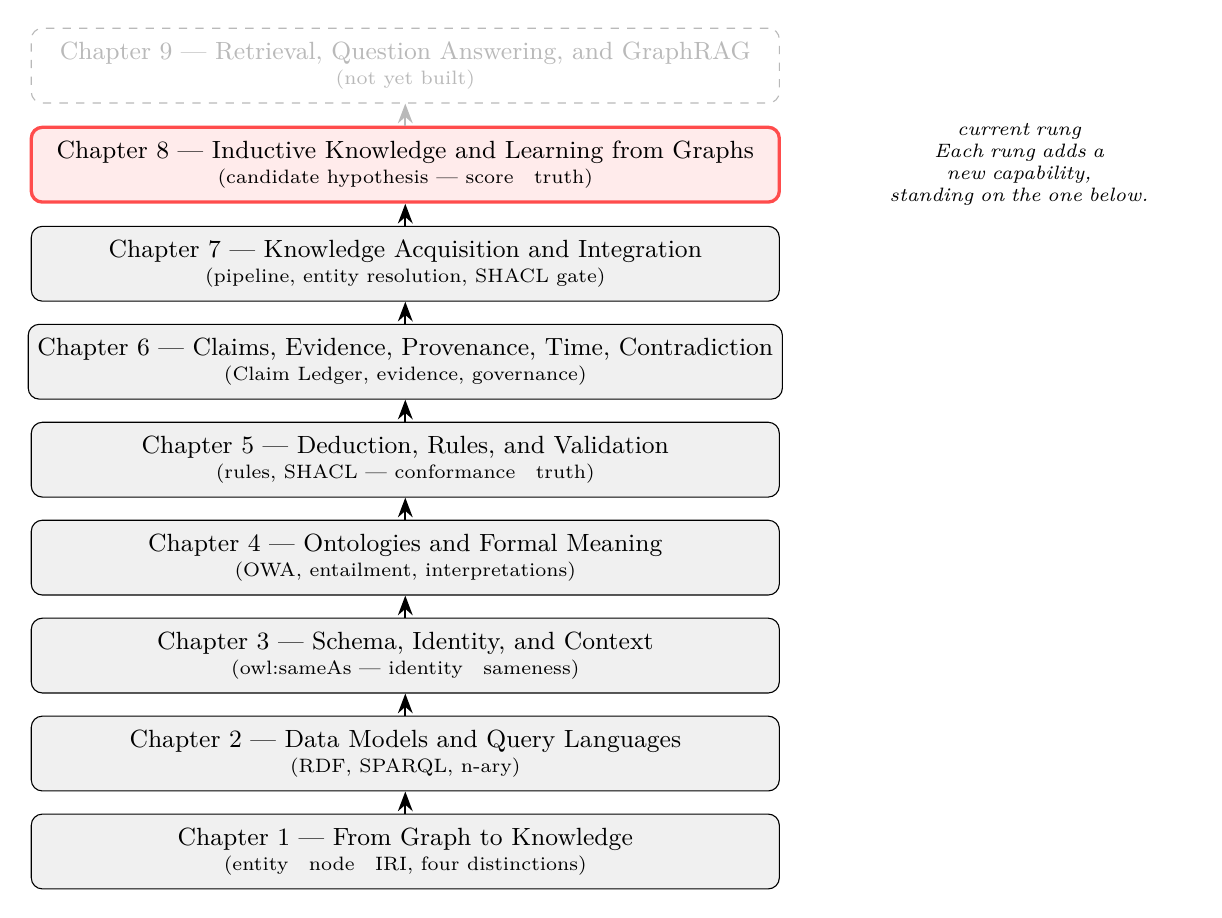
\begin{tikzpicture}[
  layer/.style={rectangle, draw, rounded corners, align=center, minimum width=9.5cm, minimum height=0.95cm, font=\small},
  arrow/.style={-{Stealth[length=2.5mm]}, thick},
  label/.style={font=\scriptsize\itshape},
]

% === Layered stack: Ch1 (bottom) → Ch8 (top) ===
\node[layer, fill=gray!12] (ch1) at (0, -0.0) {Chapter 1 — From Graph to Knowledge\\[-2pt]\scriptsize (entity ≠ node ≠ IRI, four distinctions)};
\node[layer, fill=gray!12, above=0.28cm of ch1] (ch2) {Chapter 2 — Data Models and Query Languages\\[-2pt]\scriptsize (RDF, SPARQL, n-ary)};
\node[layer, fill=gray!12, above=0.28cm of ch2] (ch3) {Chapter 3 — Schema, Identity, and Context\\[-2pt]\scriptsize (owl:sameAs — identity ≠ sameness)};
\node[layer, fill=gray!12, above=0.28cm of ch3] (ch4) {Chapter 4 — Ontologies and Formal Meaning\\[-2pt]\scriptsize (OWA, entailment, interpretations)};
\node[layer, fill=gray!12, above=0.28cm of ch4] (ch5) {Chapter 5 — Deduction, Rules, and Validation\\[-2pt]\scriptsize (rules, SHACL — conformance ≠ truth)};
\node[layer, fill=gray!12, above=0.28cm of ch5] (ch6) {Chapter 6 — Claims, Evidence, Provenance, Time, Contradiction\\[-2pt]\scriptsize (Claim Ledger, evidence, governance)};
\node[layer, fill=gray!12, above=0.28cm of ch6] (ch7) {Chapter 7 — Knowledge Acquisition and Integration\\[-2pt]\scriptsize (pipeline, entity resolution, SHACL gate)};
\node[layer, draw=red!70, very thick, fill=red!8, above=0.28cm of ch7] (ch8) {Chapter 8 — Inductive Knowledge and Learning from Graphs\\[-2pt]\scriptsize (candidate hypothesis — score ≠ truth)};

% === Future Ch9 ===
\node[layer, draw, dashed, gray!55, fill=white, above=0.28cm of ch8] (ch9) {Chapter 9 — Retrieval, Question Answering, and GraphRAG\\[-2pt]\scriptsize (not yet built)};

\draw[arrow] (ch1) -- (ch2);
\draw[arrow] (ch2) -- (ch3);
\draw[arrow] (ch3) -- (ch4);
\draw[arrow] (ch4) -- (ch5);
\draw[arrow] (ch5) -- (ch6);
\draw[arrow] (ch6) -- (ch7);
\draw[arrow] (ch7) -- (ch8);
\draw[arrow, dashed, gray!55] (ch8) -- (ch9);

% === Side annotation ===
\node[label, align=center, text width=4.2cm, right=0.8cm of ch8.east, anchor=west]
  {current rung\\ Each rung adds a\\ new capability,\\ standing on the one below.};

\end{tikzpicture}
\end{document}